\chapter{Desenvolvimento} \label{cap:desenvolvimento}

\section{Hardware}

    Para a impressão dos blocos foi utilizado a impressora 3D SnapMaker com o filamento branco no material PETG. Foi impresso uma peça nas medidas definidas no capitulo 3 para testes de material e tamanho conforme apresentado na Figura \ref{figura:teste_bloco}.
    
    \begin{figure}[H]
        \caption{Teste de tamanho e material do bloco físico}
        \centering
        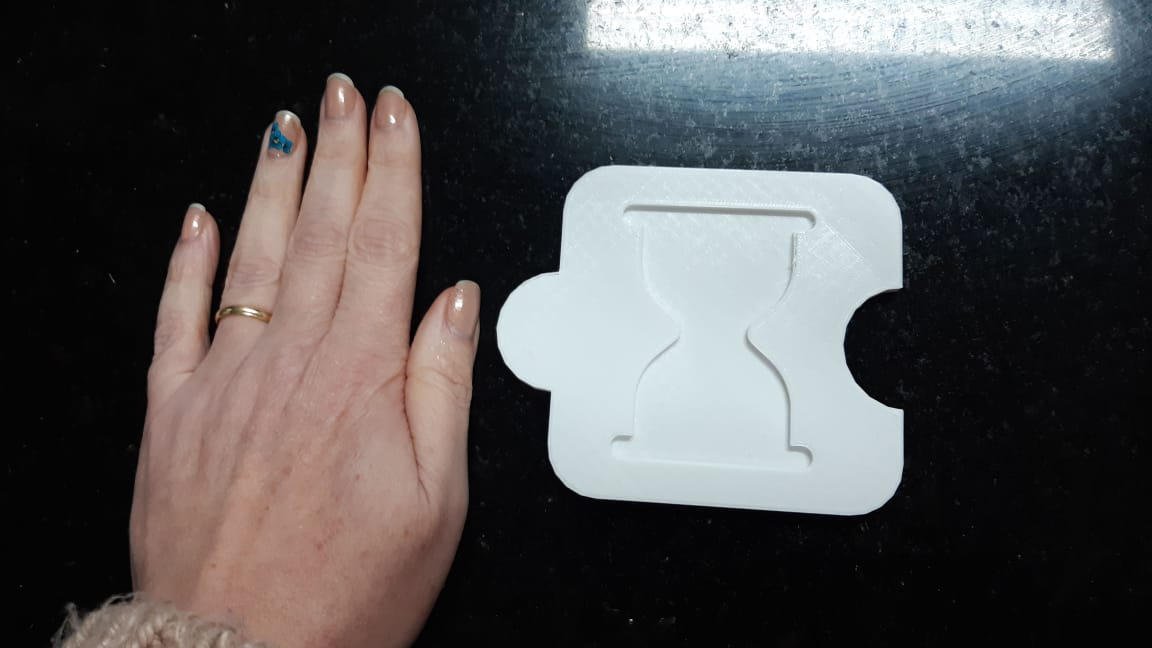
\includegraphics[width=\linewidth]{Imagens/Cap4/teste_bloco.jpeg}
        \legend{\small{Fonte: o autor (2020)}}
        \label{figura:teste_bloco}
    \end{figure}
    
    Nos testes, verificamos que o material escolhido estava dentro dos padrões aceitáveis, mantendo a peça conforme o planejado. Analisamos o tamanho da peça impressa e identificamos que estava muito grande, podendo dificultar a captura da solução pela criança. O tamanho do bloco foi reduzido para 7cm x 7cm x 5mm e um novo teste foi realizado, obtendo sucesso.
    
    Para facilitar a identificação dos blocos numéricos, alteramos o encaixe  do bloco de loop para que o bloco numérico possa encaixar lateralmente, deixando todos os blocos com encaixes laterais conforme apresentado na Figura \ref{figura:alteracao_bloco_numerico}.
    
    \begin{figure}[H]
        \caption{Alteração do bloco numérico}
        \centering
        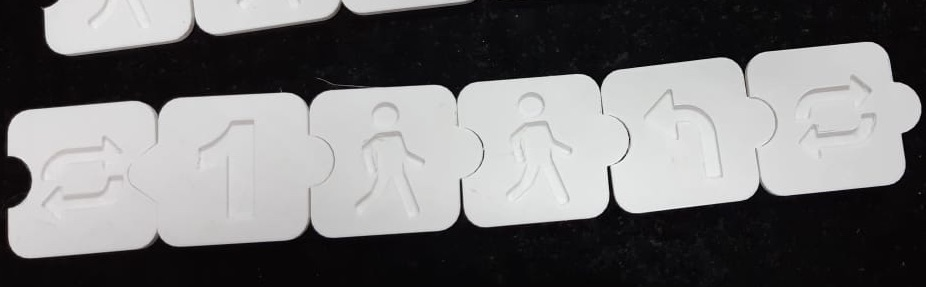
\includegraphics[width=\linewidth]{Imagens/Cap4/alteracao_bloco_numerico.jpg}
        \legend{\small{Fonte: o autor (2020)}}
        \label{figura:alteracao_bloco_numerico}
    \end{figure}
    
    As peças, impressas na cor branca, foram coloridas utilizando tinta de tecido nas cores verde, amarelo, laranja e roxo conforme apresentado na Figura \ref{figura:blocos_pintados}
    
    \begin{figure}[H]
        \caption{Alteração do bloco numérico}
        \centering
        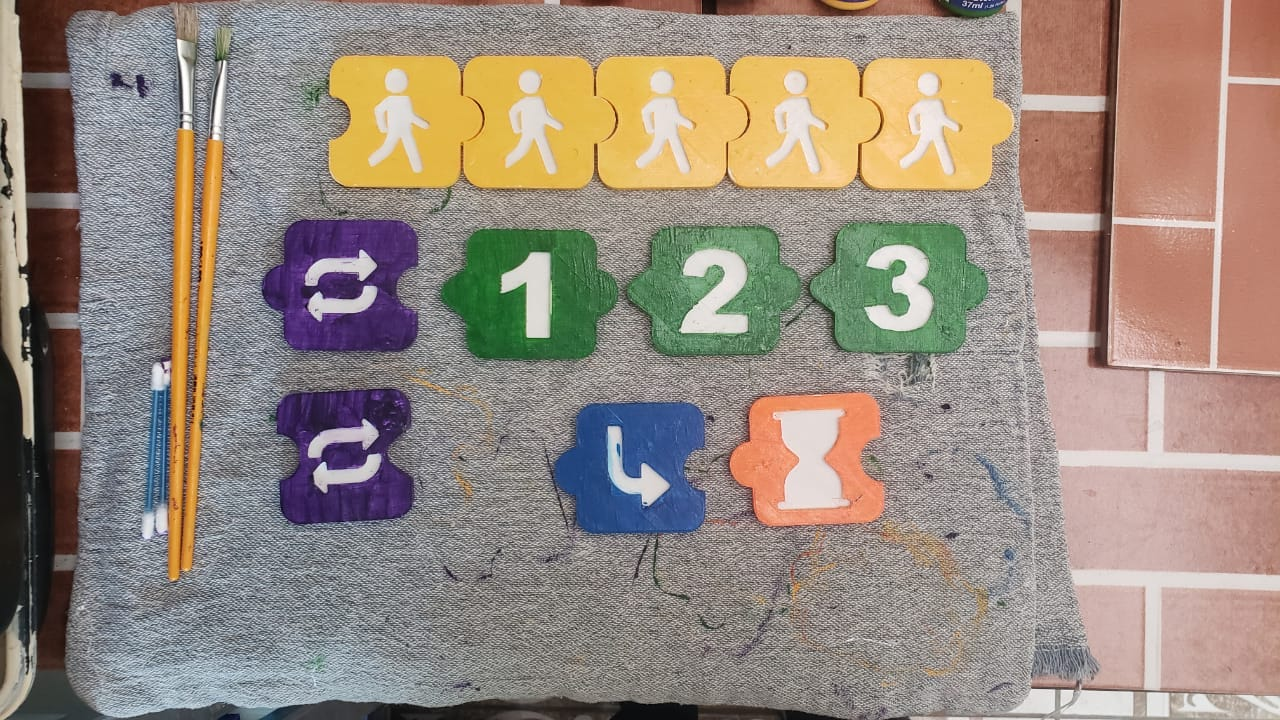
\includegraphics[width=\linewidth]{Imagens/Cap4/blocos_pintados.jpeg}
        \legend{\small{Fonte: o autor (2020)}}
        \label{figura:blocos_pintados}
    \end{figure}

\section{Software}

    \subsection{Software do jogo}
    
    \subsection{Software de reconhecimento dos blocos}
    
    \subsection{Integração dos Softwares}
    